\singlespacing
\chapter[Futuro de la aplicación]{Futuro y perspectivas de la aplicación}
\chaptermark{Futuro de la aplicación}
\onehalfspacing


\section{\textit{<<To Do>>}}

\textit{To Do} es el nombre que tradicionalmente se da en el mundo del \textit{software} a la lista tareas futuras por realizar. Todo programa informático está sometido a un interminable ciclo de vida. De él existen diferentes versiones pero ninguna se considera un trabajo <<terminado>>. \appName~ se encuentra en una primera etapa en la que tiene una arquitectura definida, tiene la capacidad de aceptar más módulos, es eficiente y su ejecución no lanza graves errores ni excepciones.

La forma más sencilla de ver el estado de implementación en el que se encuentra \appName~respecto al Synthi 100 analógico es ejecutándolo (ver \ref{ejecucion}) y observando los paneles 5 y 6, correspondientes a las matrices de \textit{audio} y \textit{voltaje} respectivamente. Por defecto, los nodos funcionales aparecen en un color más oscuro que los que aún no tienen ningún efecto. Estos paneles ofrecen así una información muy clara de qué módulos, qué entradas y qué salidas están implementadas y cuales no. Las figuras \ref{fig:nodos_enabled_audio} y \ref{fig:nodos_enabled_control} muestran el estado de implementación de \appName~en su versión \version.


\begin{figure}
	\centering
	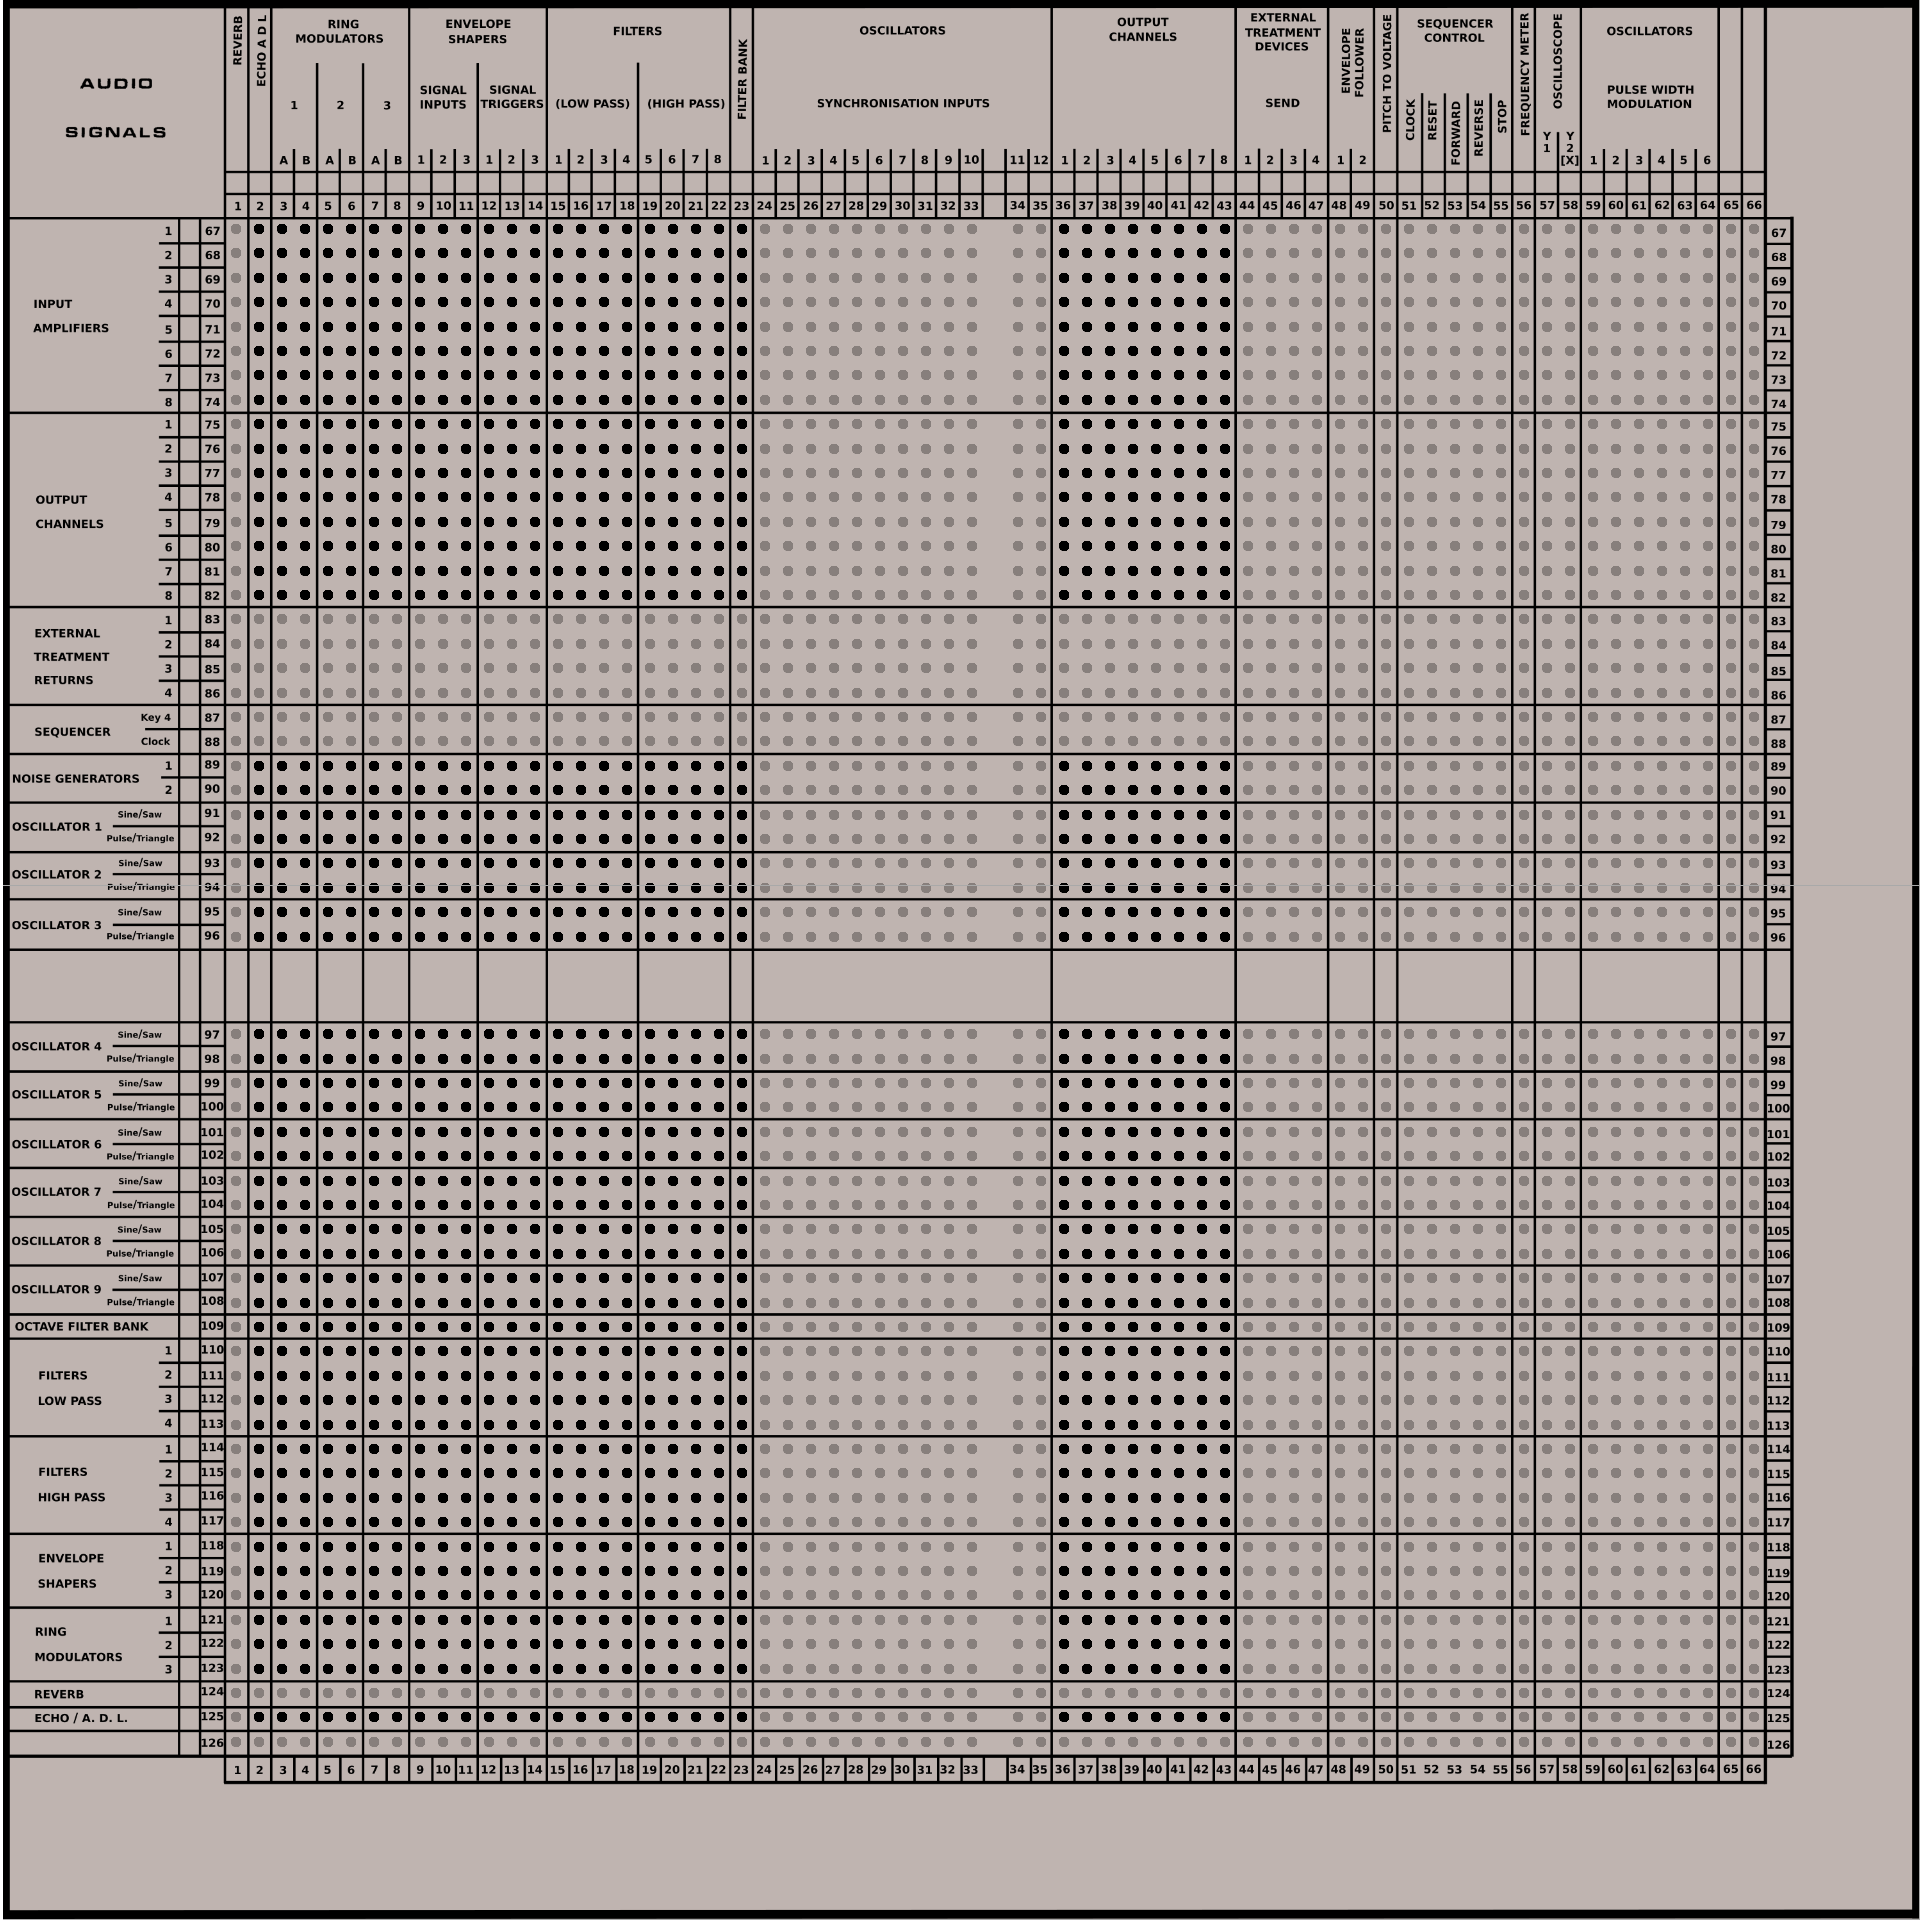
\includegraphics[width=1\textwidth]{nodos_enabled_audio}
	\caption[Módulos y nodos de \textit{audio} en funcionamiento]{Módulos y nodos de \textit{audio} en funcionamiento.}
	\label{fig:nodos_enabled_audio}
\end{figure}

\begin{figure}
	\centering
	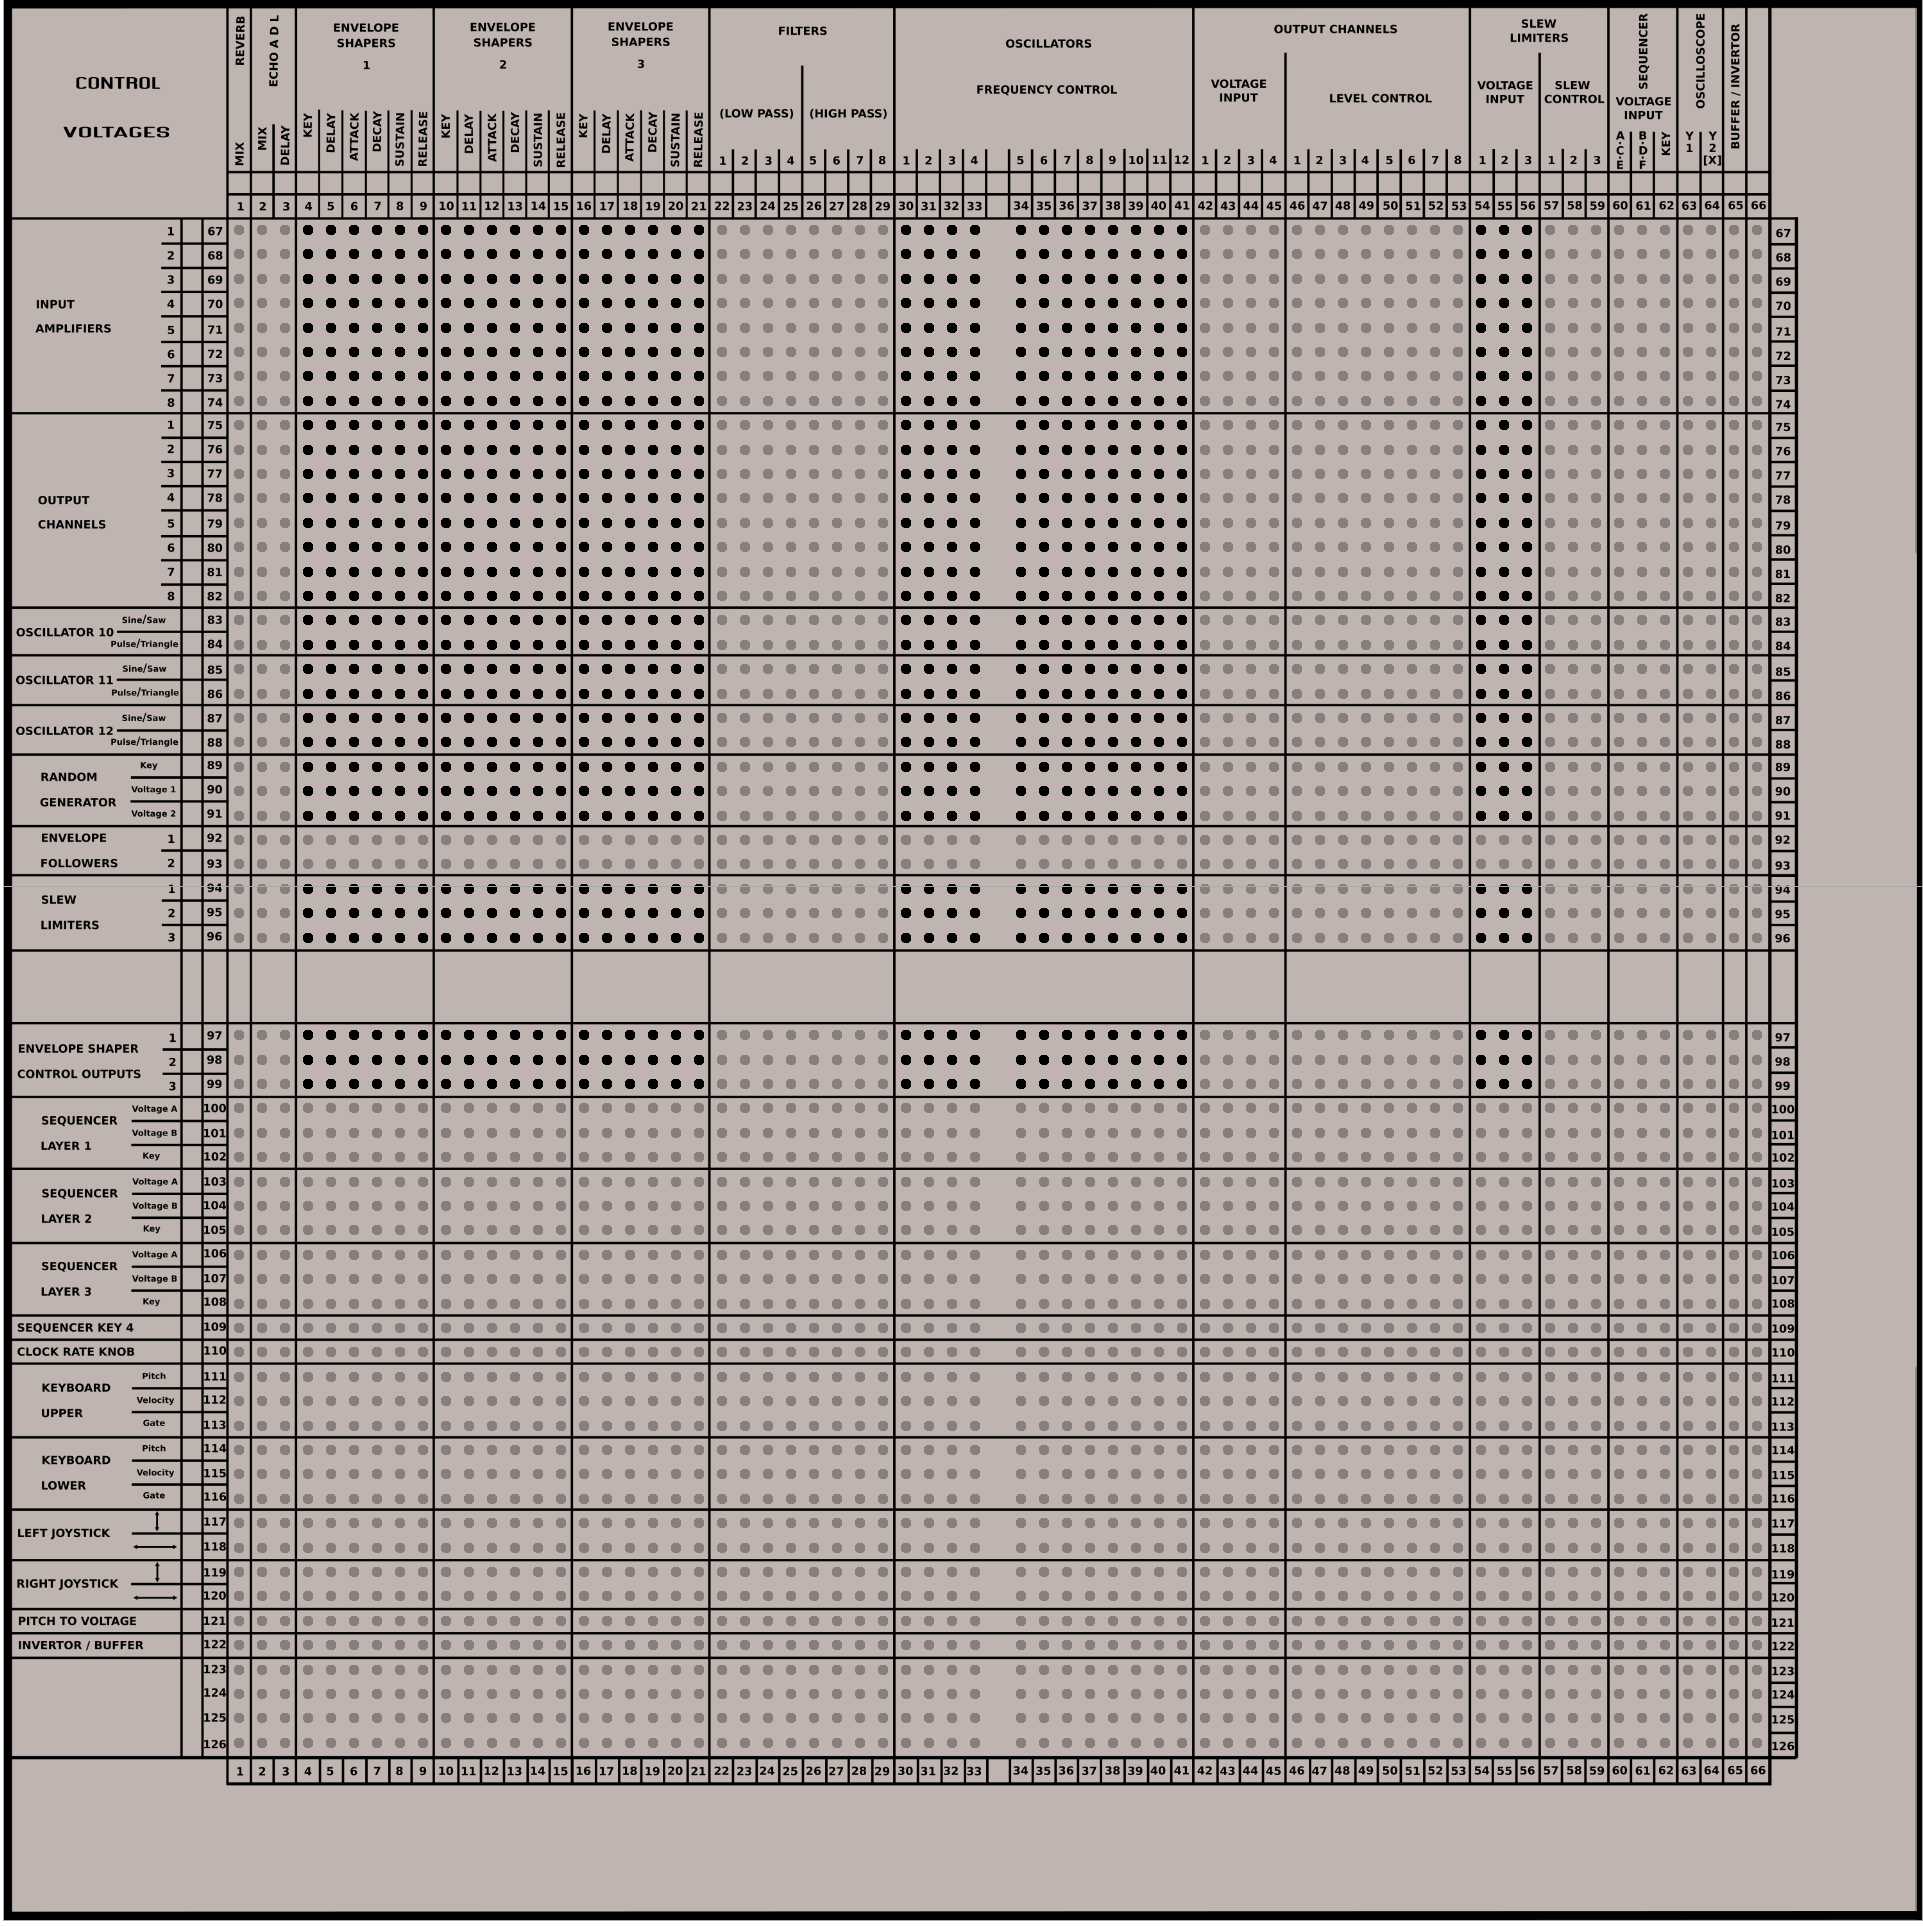
\includegraphics[width=1\textwidth]{nodos_enabled_control}
	\caption[Módulos y nodos de \textit{control} en funcionamiento]{Módulos y nodos de \textit{control} en funcionamiento.}
	\label{fig:nodos_enabled_control}
\end{figure}

\subsection{Sistema de versionado}

El número de las versiones de \appName~está compuesto de tres grupos de cifras separadas por un punto: [\textit{mayor}].[\textit{menor}].[\textit{micro}]:

\begin{description} 
	\item[\textit{mayor}] Este número cambia cada vez que hay un cambio significativo en el software.  También podría variar por la acumulación de muchos cambios menores o por razones puramente tácticas de cara a su difusión.
	\item[\textit{menor}] Se modifica cuando el software experimente cambios significativos pero que no llegan a merecer un nuevo número \textit{mayor}, como la creación de un nuevo módulo, la implementación de conexiones de audio o voltaje a un módulo, una nueva implementación de un \texttt{Synth}, etc.
	\item[micro] Este número indica cambios no significativos: refactorizaciones pequeñas, correcciones de errores no críticos, etc.
\end{description}

\appName pasará a su versión 1.0.0 en el momento de entrega de esta memoria. En el mismo repositorio de \appName~se incluirá una copia de este documento en el momento que se le asigne este número de versión.


\section{Continuación del desarrollo de \appName}


\subsection{Mejoras en el código}
Estos son los objetivos en los que se centrará el desarrollo del código de la aplicación:

\begin{enumerate}
	\item Implementar todos los módulos del Synthi 100 del GME de Cuenca.
	\item Completar todas las entradas y salidas de los módulos.
	\item Crear una interfaz de teclado MIDI para emular los dos teclados originales.
	\item Mantener el código libre de errores.
	\item Mejorar y refactorizar el código siempre que sea necesario, buscando la legibilidad y la eficiencia.
	\item Simplificar al máximo las dependencias de software, como \textit{sc3-plugins}.
	\item Acceder al Synthi 100 de Cuenca con el fin de obtener muestras para estudiar el comportamiento de los diferentes módulos de cara a una implementación más fiel.
\end{enumerate}


\subsection{Interacción con el usuario}
De cara a al usuario y la usabilidad de la aplicación:

\begin{enumerate}
	\item Crear de ejecutables \textit{standalone} para las tres plataformas de escritorio (Mac Os, Windows y Linux).
	\item Testar en profundidad y obtener \textit{feedback} de los usuarios.
	\item Mejorar la interfaz para que sea intuitiva.
	\item Sustituir las fotografías actuales por unas de alta calidad.	
\end{enumerate}


\subsection{Difusión, formación e información}

Este apartado es muy importante de cara al éxito de la aplicación. Los esfuerzos se centrarán en los siguientes puntos:

\begin{enumerate}
	\item Creación de un conjunto de videotutoriales de uso de \appName.
	\item Ofrecer la posibilidad de charlas y talleres divulgativos en torno a \appName~o la programación en SuperCollider.
	\item Completar la documentación en Supercollider.
\end{enumerate}

